\documentclass[10pt]{beamer}
\setbeamertemplate{navigation symbols}{\insertlogo}

%\documentclass[handout,dvips,11pt,grey]{beamer}

%\usetheme{Goettingen}
%\usetheme{Warsaw}
\usetheme{Hannover}

%\usepackage{tikz,pgf}
\usepackage{xcolor}
\usepackage{multicol}
\usepackage{amsmath,amsthm,amssymb}
%\usepackage{epstopdf}
\usepackage{xspace}
\usepackage{wrapfig}

\usepackage{verbatim}
%\usepackage{circuitikz}
%\usepackage{graphicx}
\usepackage{comment}
%\usepackage{array}
\usepackage{coffee4}

\title{Understanding and Using Topic Modeling}
\subtitle{Using inferred document clusters}
\author{Philip Robinson}
\date{\today}
\institute{Presented to OpsLab \\ NASA - Jet Propulsion Lab}

\DeclareMathOperator*{\argsort}{argsort}

  \logo{
\includegraphics[height=.7cm]{./logo.png}}

\begin{document}

\begin{frame}
  \titlepage

\end{frame}

\section{Introduction}
\begin{frame}{Introduction - Philip (1762)}
  Computer Science MSc at Oregon Health and Science University.

  \vspace{1em}

  \begin{multicols}{2}
    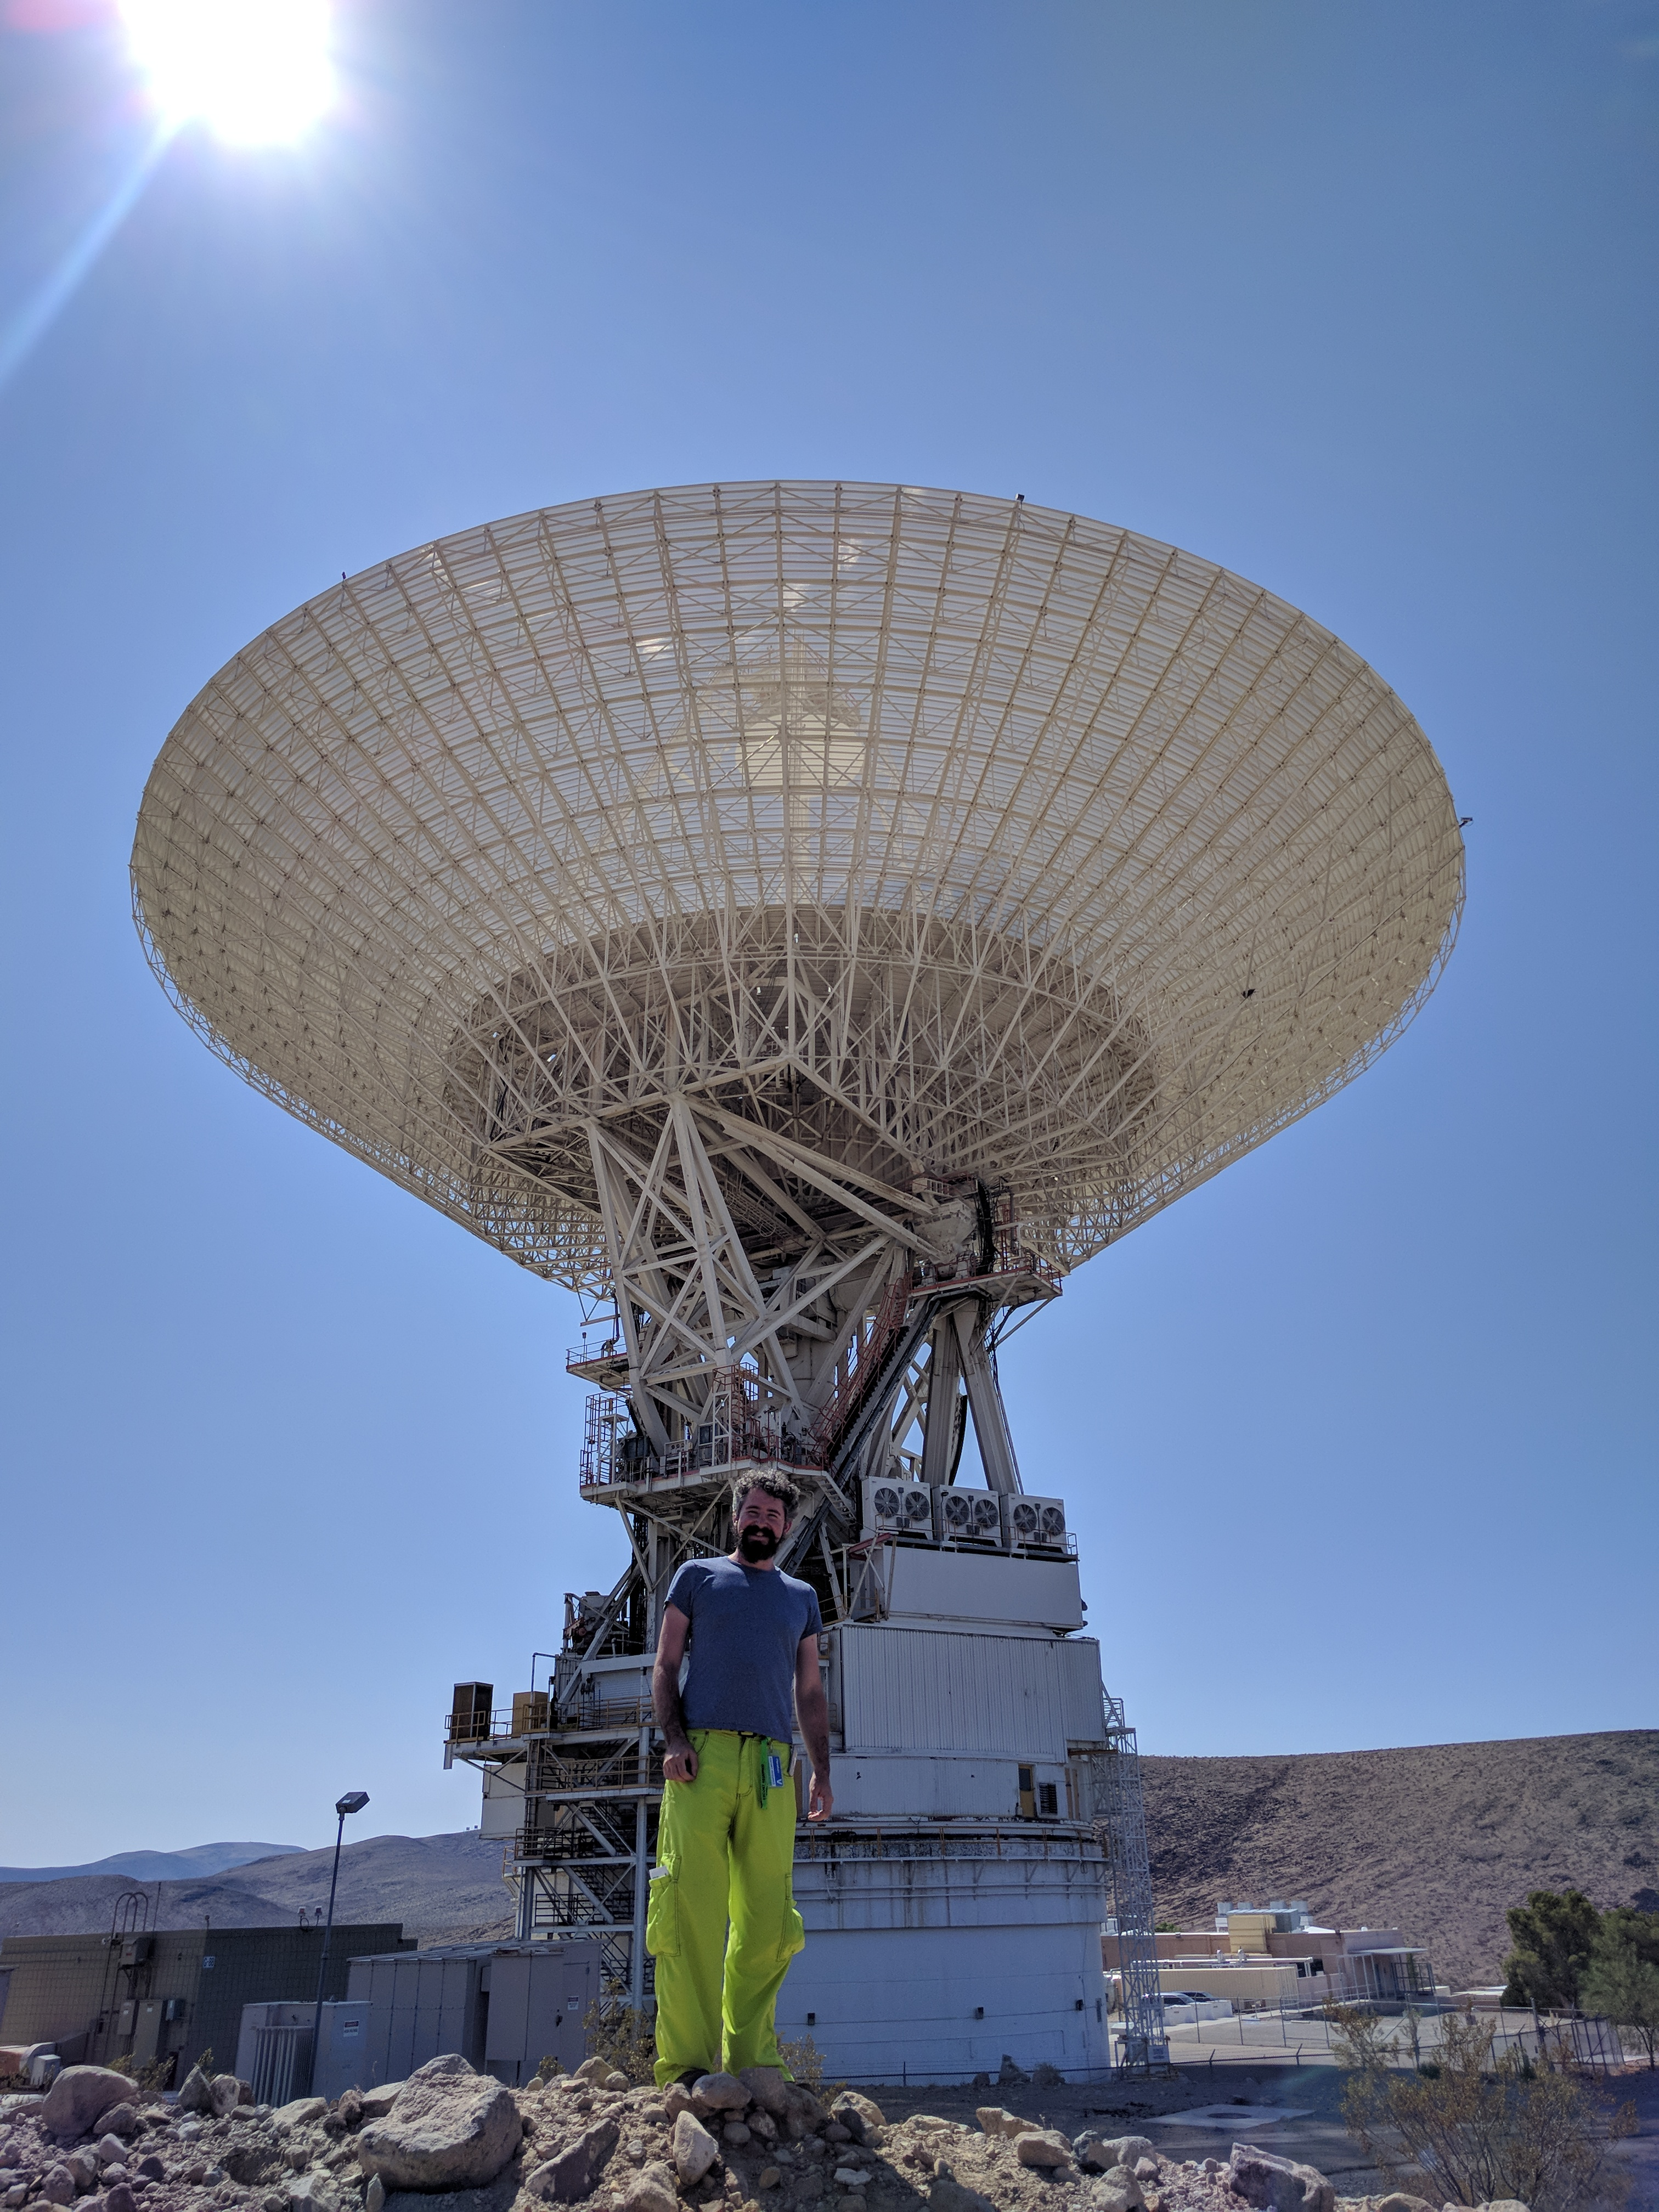
\includegraphics[width=\columnwidth]{./philip.jpg}


  \begin{itemize}
  \item Whale vocalization
  \item Light pollution
  \item Modern cryptography
  \item[$\star$] Information retrieval
  \end{itemize}

  \end{multicols}

\end{frame}

\begin{frame}{Presentation Overview}
  \tableofcontents

\end{frame}

\section{What is Topic Modeling}

\begin{frame}{What is Topic Modeling}
  \begin{quote}
    Topic modeling is a text processing technique for automatically grouping documents by topics. This is usually used as a strategy to describe documents in low dimensional space or an exploratory tool for document collections.
  \end{quote}
\end{frame}

\newcommand{\Food}[1]{\colorbox{orange!30}{#1}\xspace}
\newcommand{\Travel}[1]{\colorbox{blue!30}{#1}\xspace}
\newcommand{\Time}[1]{\colorbox{green!30}{#1}\xspace}
\newcommand{\Document}[1]{\fbox{\begin{minipage}{\columnwidth}#1\end{minipage}}}



\begin{frame}{Examples}
{\bf In practice, this requires many more documents}

  \begin{multicols}{2}

    \Document{
      The \Travel{Tourist} huddles in the \\ \Travel{station} While slowly \Time{night} gives way to \Time{dawn}; He finds a certain fascination In knowing all the \Travel{trains} are gone.
    }

    \vspace{.25em}

    \Document{
      The Governess up in the attic \\Attempts to make a cup of \Food{tea}; Her mind grows \Time{daily} more erratic From cold and \Food{hunger} and ennui.
    }

    \vspace{.25em}

    \Document{
      The Journalist surveys the slaughter, The best in \Time{years} without a doubt; He pours himself a \Food{gin} and \Food{water} and wonders how it came about.
    }

    \columnbreak

    \begin{itemize}
    \item \Food{Food}
    \item \Travel{Travel}
    \item \Time{Time}
    \end{itemize}

    \vspace{1em}

    From this annotation we know that Document 2 and 3 are about \Food{Food} and \Time{Time}
  \end{multicols}

\end{frame}

\section{Why Topic Model}

\begin{frame}{What can I solve?}
  \begin{itemize}
  \item Find similar document pairs
  \item Cluster documents into groups with similar content
  \item Find relevent documents to a query or user's interests
  \item Explore shape of document collection
  \item Can be extended to address many other problems
  \end{itemize}
\end{frame}

\begin{frame}{Applications of Topic Modeling}

  \begin{multicols}{3}

  \begin{figure}
  \includegraphics[width=\columnwidth]{full2.png}
  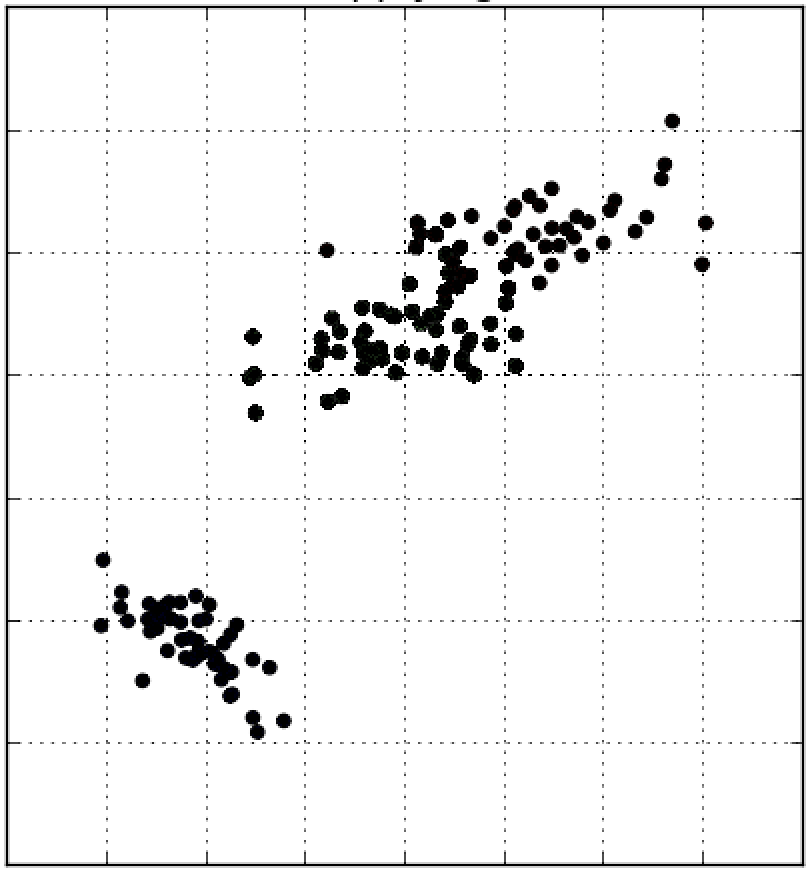
\includegraphics[width=.8\columnwidth]{reduced.png}
  \caption{Dimmentionality Reduction}
  \end{figure}

  \columnbreak

  \hfill
    \begin{figure}
  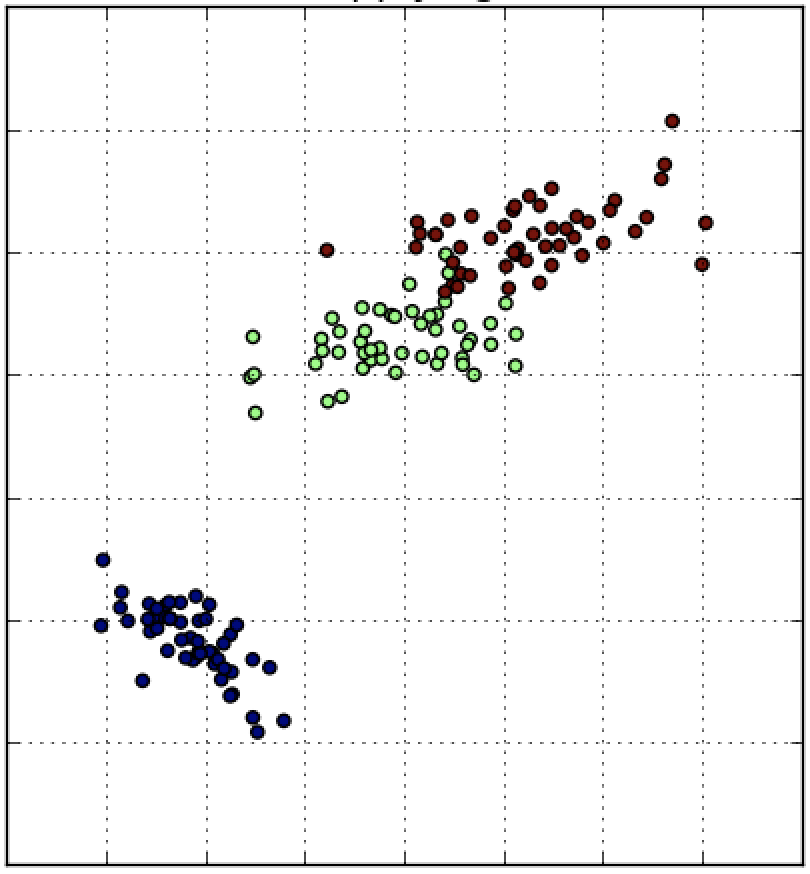
\includegraphics[width=\columnwidth]{cluster.png}
  \caption{Cluster Points}
  \end{figure}

    \columnbreak

  \hfill
    \begin{figure}
  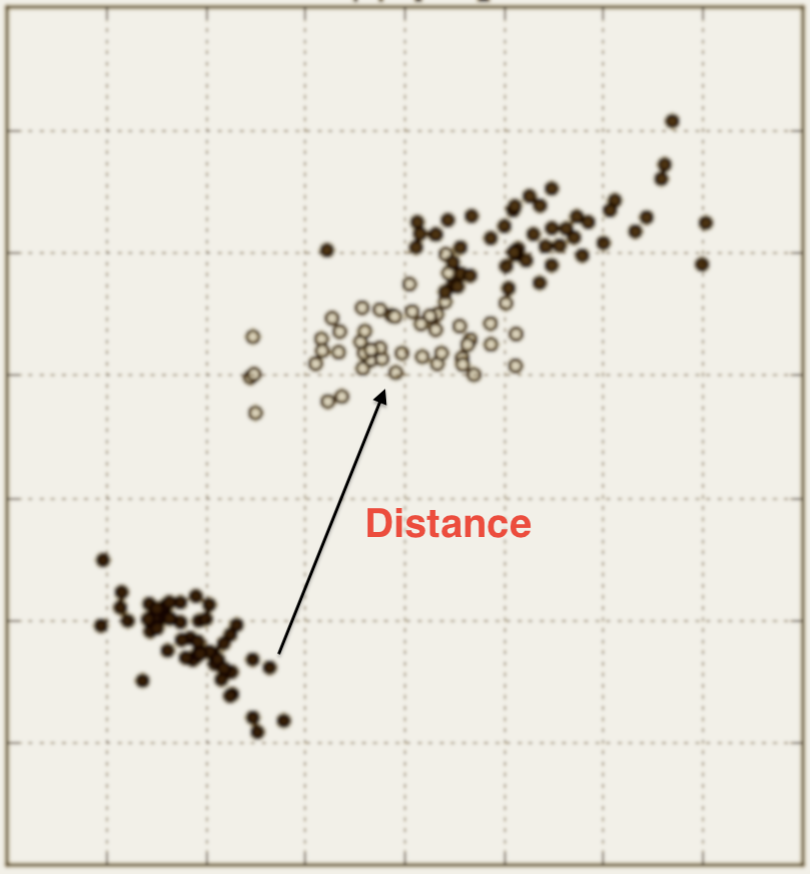
\includegraphics[width=\columnwidth]{dist.png}
  \caption{Exploratory Data Analysis}
  \end{figure}

  \end{multicols}

\end{frame}

\section{A Generative Model}

\begin{frame}{Latend Dirichlet Allocation (LDA)}
  {\bf A generative model}

  \begin{itemize}
  \item Assume/Generalize how documents could have been generated
  \item Fit parameters that describe generalization
  \item Ask questions about the generalization in relation to documents
  \item Ask questions about documents in relation to the generalization
  \end{itemize}

  \vspace{1em}

  Topic modeling generalizes how a document is generated by claiming that words come from topics, and documents have multiple topics. Note that this ignores sentence structure, entities, authorship, or other things we may care about.
\end{frame}


\begin{frame}{Topic Modeling}

  \begin{multicols}{2}

  \begin{itemize}
  \item Represent document as Bag-of-Words\footnote{equivelent to multinomial over the vocabulary}
  \item Model/Fit topics as mixture of words
  \item Documents are projected into topic space
  \item Study relationships between document projections
  \end{itemize}

  \begin{figure}
  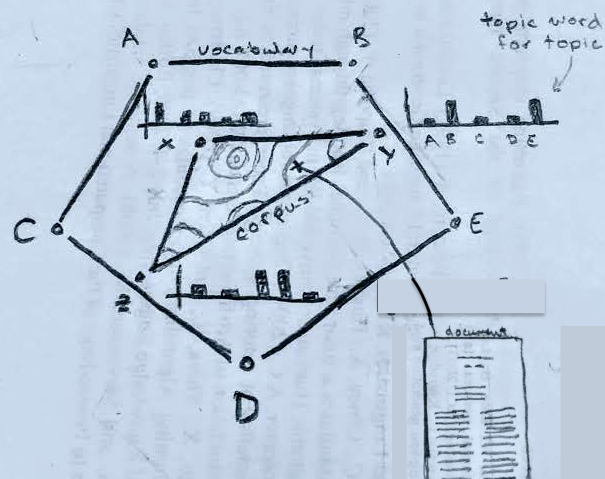
\includegraphics[width=\columnwidth]{./lda-draw.png}
  \caption{Latent Dirichlet Allocation}
  \end{figure}

  \end{multicols}

  \begin{align*}
    T(x) &= \texttt{Project $x$ into topic-space} \\
    Measure &= Distance(T(\texttt{Doc 1}),T(\texttt{Doc 2}))
  \end{align*}

\end{frame}

\section{Understanding Model Space}

\begin{frame}{Dirichlet Distribution}
  {\bf In this case the Topic-Space is our Dirichlet Distribution}

    \begin{multicols}{3}

  \begin{figure}
  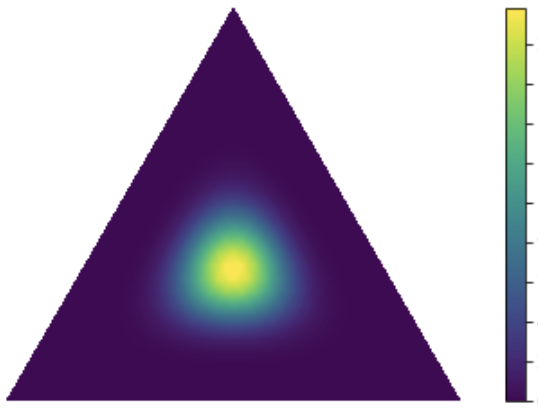
\includegraphics[width=\columnwidth]{uninformative}
  \caption{Non-Informative}
  \end{figure}

  \columnbreak

  \hfill
    \begin{figure}
  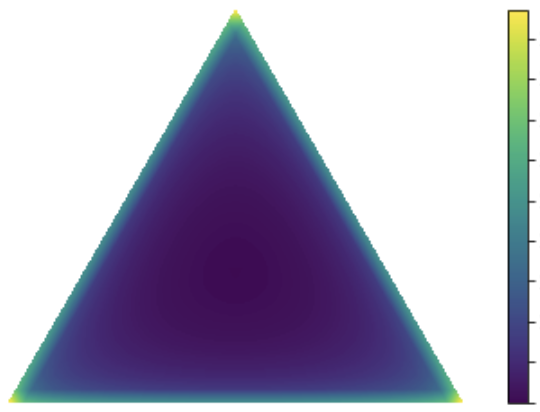
\includegraphics[width=\columnwidth]{unique.png}
  \caption{Little In Common}
  \end{figure}

    \columnbreak

  \hfill
    \begin{figure}
  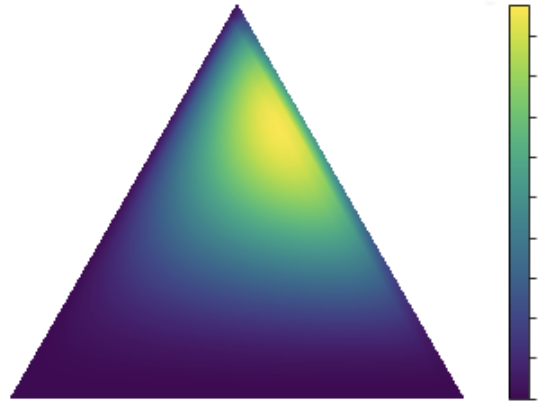
\includegraphics[width=\columnwidth]{shared.png}
  \caption{Shared Topics}
  \end{figure}

  \end{multicols}

\end{frame}

\begin{frame}{Using this in Python\footnote{example in \texttt{scikit-learn}, I used \texttt{gensim}}}
  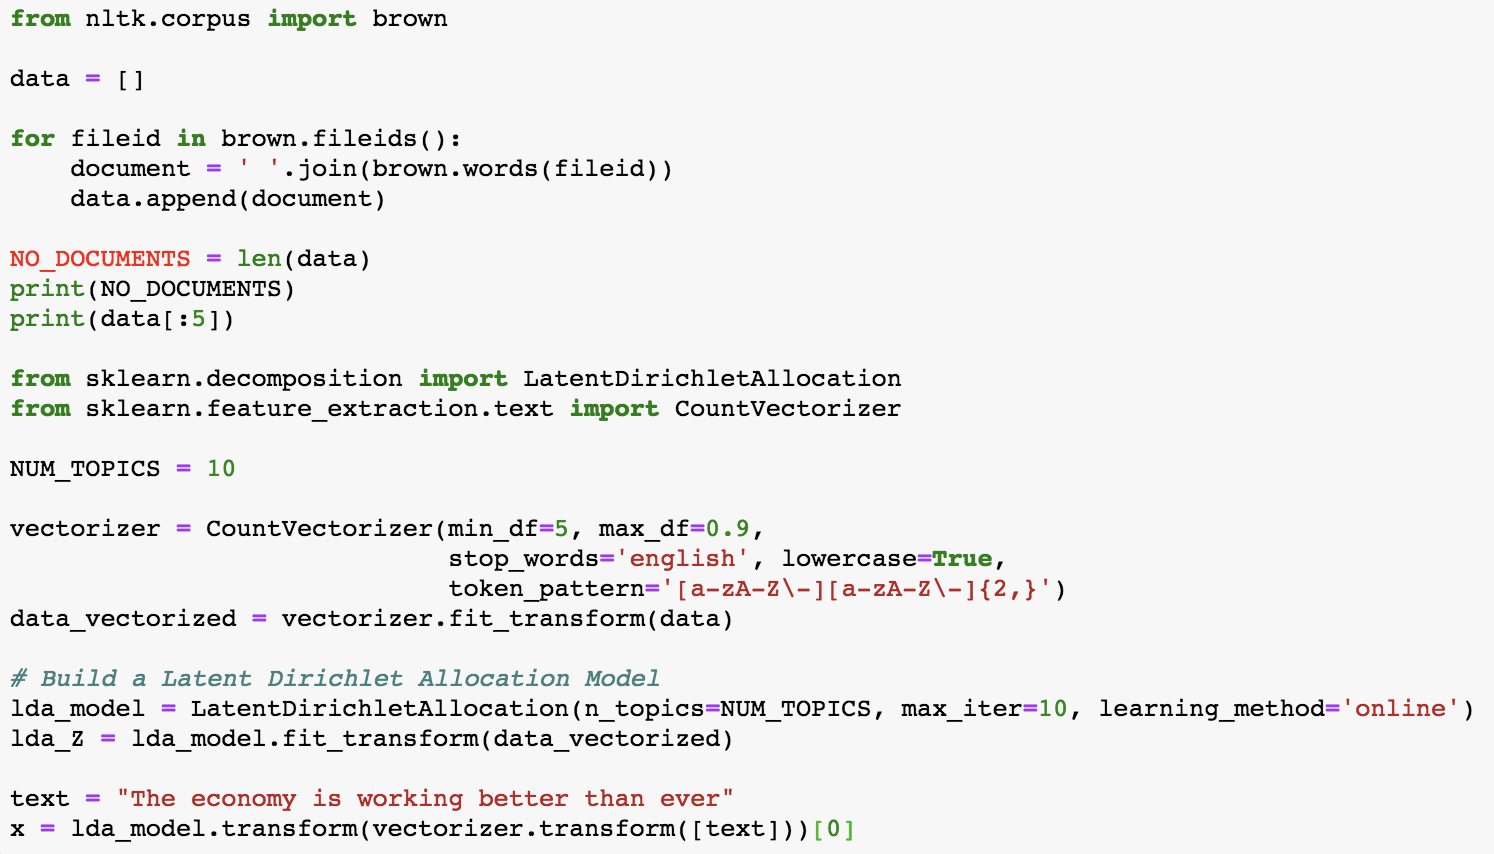
\includegraphics[width=\textwidth]{./implement.png}
\end{frame}



\section{Details}

\begin{frame}{Concerns about Topics}
  \begin{itemize}
  \item Topics do not have labels
  \item Topics are not easily human interpretable
  \item In traditional LDA n-grams are not represented
  \end{itemize}
\end{frame}

\begin{frame}{Visualizing High Dimensional Space\footnote{used \texttt{pyLDAvis}}}

    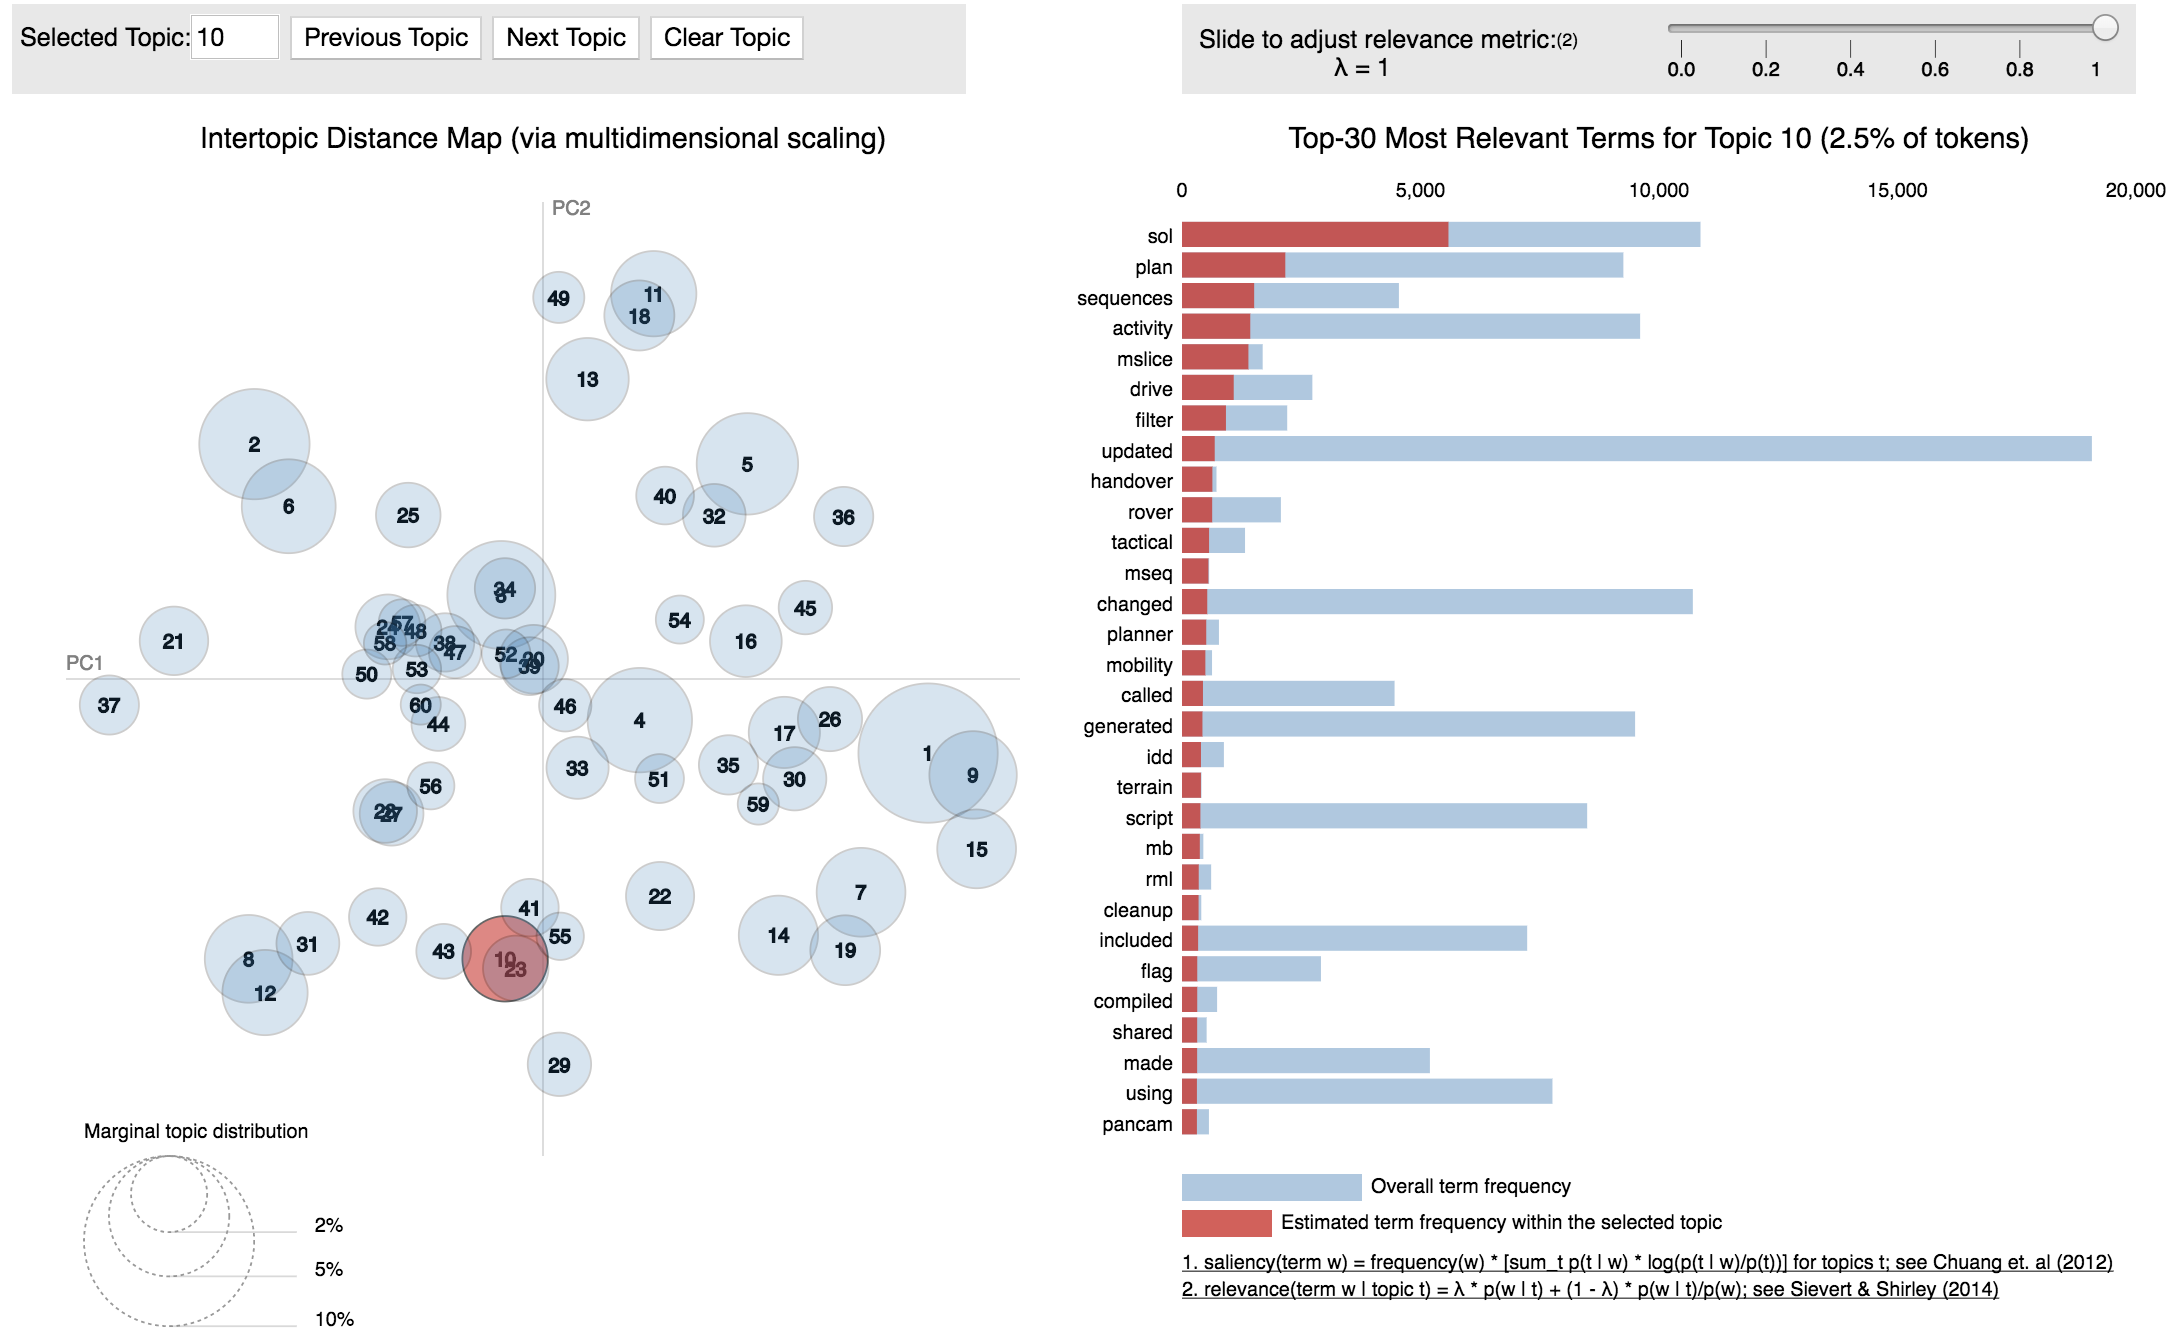
\includegraphics[width=\textwidth]{LDAvis.png}

\end{frame}

\begin{frame}{Looking at Topics}

  {\centering Breakout to Jupyter}
\end{frame}


\begin{comment}

  \section{Preping Text}

\begin{frame}{Text Pre-Processing}

  ATM is a derivative of Latent Dirichlet Allocation (LDA), which is a generative \texttt{bag-of-words} model for producing topics described as a mixture of words.

  \begin{itemize}
  \item Join all Free Text fields
  \item Lowercase text
  \item Remove non-informative text patterns
  \item Stem \hfill\texttt{(applies, applying, apply) -> (appli)}
  \item Un-Stem \hfill\texttt{(appli) -> (apply)}
  \item Identify and remove ``Stop Words''
    \begin{itemize}
    \item most frequent .06\% (empirical choice)
    \item \texttt{nltk} english stop-words
    \end{itemize}
  \item Remove rare words
  \end{itemize}

\end{frame}
\end{comment}

\section{Notes}

\begin{frame}{Evaluation Notes}

  As this is a bayesian machine learning approach we will need to evaluate model fit.

  \begin{itemize}
  \item perplexity
  \item coherence
  \item visualization
  \item predictive power
  \end{itemize}
\end{frame}

\begin{frame}{Preprocessing Notes}
  As this model generates conditional probabilities on observed words, we need a clean/normalize vocabulary

  \begin{itemize}
  \item Lowercase corpus
  \item Tokenization \& (Stemming | Lemmatization)
  \item Removing symbols
  \item Remove highly common words
  \item Remove extreamly rare words
  \end{itemize}
\end{frame}

\section{Conclusion}

\begin{frame}{Conclusion \& Questions}

  \begin{quote}
    I used this technique during my internship to automatically assign tickets to subject matter experts, for the Office of Safety and Mission Success (5x)\footnote{1762 acts as data science support to JPL}
  \end{quote}

\end{frame}

\end{document}
